% Dummy comment so that files shows up in Reviewable.
Recall that in Section~\ref{sec:unconstrained_convex_formulation}
we defined \emph{Inverse Dynamics}
as the construction of the optimal dual impulses
from the optimal primal velocities.  As shown in~\cite{bib:todorov2014},
these impulses have formula $\bgamma = P_{\mathcal{F}}(\vf{y})$, 
where $P_{\mathcal{F}}$ denotes projection
with respect to the weighted norm $\|\cdot\|_{\mf R}$, i.e.,
\[
P_{\mathcal{F}}(\vf{y}) = \argmin_{\bgamma\in\mathcal{F}} \quad \frac{1}{2}(\bgamma-\vf{y})^T\vf{R}(\bgamma-\vf{y}).
\]
We next show this projection is easily computed
if one first applies a change of variables and works with the usual Euclidean norm $\|\cdot\|$.


To ease notation, we consider the case where $\mathcal{F}$
is a single friction cone $\mathcal{F}_{\mu} \in \mathbb{R}^3$
and $\mf{R}$ is the diagonal matrix $diag(R_n, R_t, R_t)$
for $R_n, R_t \in \mathbb{R}$.  For the general setting, projection
onto $\mathcal{F}_{\mu_1} \times \mathcal{F}_{\mu_2} \cdots \mathcal{F}_{\mu_{n-1}}\times\mathcal{F}_{\mu_n}$
can be done  by applying the provided formula to
each cone $\mathcal{F}_{\mu_i}$ individually.

To begin, we let $\tilde\bgamma=\vf{R}^{1/2}\bgamma$ 
and rewrite $P_{\mathcal{F}}(\vf{y})$ as
\[
  P_{\mathcal{F}}(\vf{y}) = \mf{R}^{-1/2} \argmin_{\tilde \bgamma\in \mf{R}^{1/2} \mathcal{F}} \quad \Vert\tilde\bgamma-  \vf{R}^{1/2}\vf{y} \Vert_2^2
\]                                                                               
Observing that $\mf{R}^{1/2} \mathcal{F}_{\mu} = \mathcal{F}_{\tilde\mu}$ for $\tilde \mu =\mu\,(R_t/R_n)^{1/2}$,
we conclude that
\begin{eqnarray}
  P_\mathcal{F}(\vf{y})=\vf{R}^{-1/2} \tilde{P}_\mathcal{F_{\tilde\mu}}(\vf{R}^{1/2}\vf{y})
	\label{eq:local_optimization_problem_tilde}
\end{eqnarray}
where $\tilde{P}_\mathcal{F_{\tilde\mu}} : \mathbb{R}^3 \rightarrow \mathbb{R}^3$ denotes Euclidean projection onto $F_{\tilde\mu}$.

A simple piecewise formula for evaluating $\tilde{P}_\mathcal{F_{\tilde\mu}}$ 
is obtained by partitioning its domain  into three regions.
This partition consists of the cone $\mathcal{F}_{\tilde\mu}$, which we call \textit{Region I},
the interior of the polar $\mathcal{F}_{\tilde\mu}^\circ$, which we call \textit{Region II},
and the remaining area, which we call \textit{Region III}.
In Region I, we simply have that $\tilde P_\mathcal{F_{\tilde\mu}}(\tilde{\vf{y}}) = \tilde{\vf{y}}$.
In Region II, $\tilde P_\mathcal{F_{\tilde\mu}}(\tilde{\vf{y}}) = 0$.
Finally, in Region III, we evaluate $\tilde P_\mathcal{F_{\tilde\mu}}(\tilde{\vf{y}})$
via Euclidean projection onto the boundary of $\mathcal{F}_{\tilde\mu}$,
which admits a simple formula. 
Indeed, we have that 
$\tilde P_\mathcal{F_{\tilde\mu}}(\tilde{\vf{y}}) = (\tilde{\bgamma}_t, \tilde{\gamma}_n)$,
where
\begin{align}\label{eq:ProjectionFormula}
\begin{aligned}
  \tilde{\bgamma}_t       &= \tilde{\mu}\tilde{\gamma}_n\hat{\vf{t}}\\
        \tilde{\gamma}_n  &= \frac{1}{1+\tilde{\mu}^2}\left(\tilde{y}_n +
	\tilde{\mu}\tilde{y}_r\right)
\end{aligned}
\end{align}
and $\hat{\vf{t}}=\vf{y}_t/\Vert\vf{y}_t\Vert$. 
Observe in Fig.~\ref{fig:cone_regions} that  $\tilde\mu$ is precisely the tangent of the angle $\theta$ between the boundary 
of $\mathcal{F}_{\tilde\mu}$ and the vertical axis,
whereas $1/(1+\tilde\mu^2)$ is its cosine. \fbox{The figure suggests it is $\cos^2 \theta$. 
Which is correct?}. Also
note that this formula is well-defined on Region III,
since $\vf{y}_t = 0$ only if $\vf{y}$ is
lies in Regions I or II.




\begin{figure}[!h]
    \centering
    %\vspace{6pt}
    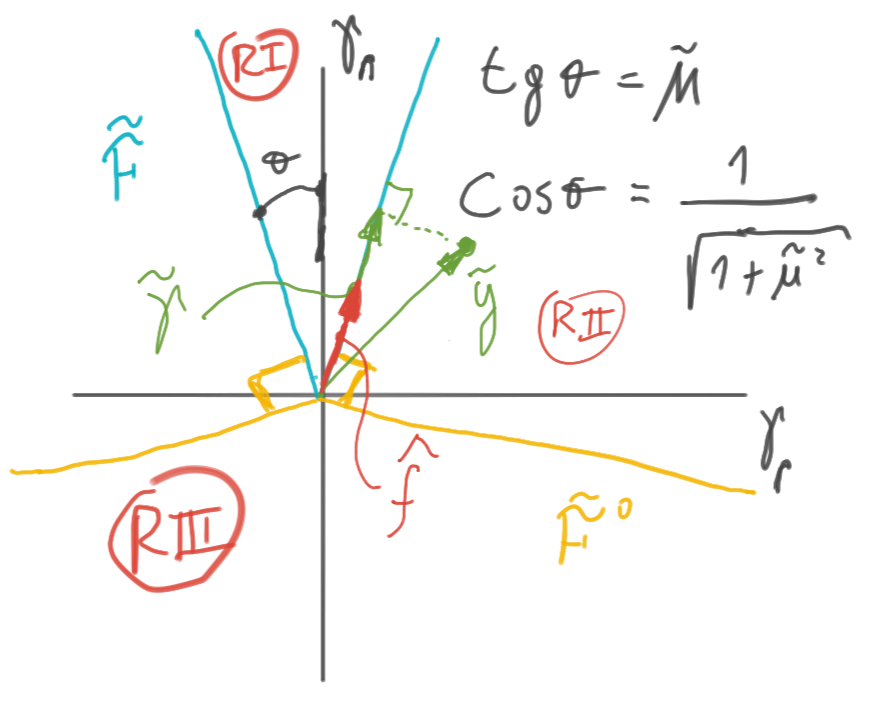
\includegraphics[width=0.45\columnwidth]{figures/cone_regions.png}
    \caption{Geometry of $\mathcal{F}_{\tilde\mu}$ and regions in the
    $\tilde{\vf{y}}$ space.}
    \label{fig:cone_regions}
\end{figure}
In total, for $\mathcal{F} = \mathcal{F}_{\mu}$, we obtain the projection $\bgamma = P_\mathcal{F}(\vf{y})$  by setting 
$\tilde{\vf{y}} = \mf{R}^{1/2} \tilde{\vf{y}}$, computing $\tilde\bgamma$ from
the formula~\eqref{eq:ProjectionFormula} and applying the inverse transformation $\bgamma=\mf{R}^{-1/2}\tilde\bgamma$.
%to recover the impulses projected onto the
%friction cone ${\mathcal{F}}_{\mu}$ using the norm in $\vf{R}$.

% Not sure that these adds anything
%Though the tangent vector $\hat{\vf{t}}$ is not defined for $\vf{y}=\vf{0}$, the
%projection still is, $P_\mathcal{F}(\vf{0})=\vf{0}$. In practice however, we
%introduce a smooth \emph{soft-norm} defined as
%$\|\vf{x}\|_s=\sqrt{\|\vf{x}\|^2+\varepsilon_s^2}$ and we define the tangent
%vector as $\hat{\vf{t}}=\vf{y}_t/\Vert\vf{y}_t\Vert_s$. This newly defined tangent vector is smooth and has the desired property that it leads to the right
%projection result in the limit to $\vf{y}\rightarrow 0$. In addition, not only
%the projection is well defined, but also its gradients in Appendix
%\ref{app:gradients_derivation}. In practice we use $\varepsilon_s=10^{-8}$.

